% https://de.overleaf.com/latex/templates/a-quick-guide-to-latex/fghqpfgnxggz

\documentclass[10pt]{article}
% ========== Packages ==========
\usepackage[a4paper,
  left=10mm,
  right=10mm,
  top=10mm,
  bottom=17mm
]{geometry}

% \usepackage[ngerman]{babel} %Ändert die Sprache
\usepackage[T1]{fontenc} %Wichtig für ä ö ü
\usepackage{amssymb,amsmath,amsthm,amsfonts}
\usepackage{graphicx}
\usepackage{fancyhdr}
\usepackage[utf8]{inputenc}
\usepackage{multicol,multirow}
\usepackage{longtable} %Für lange Tabellen
\usepackage{arydshln} %Für gestrichelte Linien in Tabellen
\usepackage{tabularx}
\usepackage{pdfpages} %Zum einfügen von PDF's
\usepackage{hyperref} %Für hyperlinks
\hypersetup{bookmarks=true}
\usepackage{parskip}
\usepackage{caption} %Für die Beschriftung von Bilder
\captionsetup{justification=centering}
\captionsetup{font=it}
\setlength{\parindent}{0pt}
\usepackage{subcaption} %Für die Beschriftung unterteilter Bilder
\usepackage{float}
\floatstyle{plaintop}
\restylefloat{table}
\usepackage{siunitx}%Für einheiten im Symbolverzeichnis
% \usepackage[symbols,nogroupskip,sort=none]{glossaries-extra}%Für Symbolverzeichnis
% % \input{symbolverzeichnis}
\usepackage{lipsum}%Für pseudo text



\makeatletter %Für römische Zahlen
\newcommand*{\rom}[1]{\expandafter\@slowromancap\romannumeral #1@}

%Für die dicken Linien in Tabellen
\def\thickhline{%
  \noalign{\ifnum0=`}\fi\hrule \@height \thickarrayrulewidth \futurelet
   \reserved@a\@xthickhline}
\def\@xthickhline{\ifx\reserved@a\thickhline
               \vskip\doublerulesep
               \vskip-\thickarrayrulewidth
               \fi
      \ifnum0=`{\fi}}
\makeatother
\newlength{\thickarrayrulewidth}
\setlength{\thickarrayrulewidth}{2\arrayrulewidth}

%Sorgt dafür, dass nicht immer alles auf die ganze Seite verteilt wird.
\raggedbottom

% ========== Header and Footer ==========
\pagestyle{fancy}
\fancyhf{}
% \fancyhead[RE,LO]{Seite \thepage}
% \fancyhead[LE,RO]{\nouppercase{\leftmark}}
\fancyfoot[RE,LO]{Page \thepage}
\renewcommand{\headrulewidth}{0pt}
\renewcommand{\footrulewidth}{.5pt}

%Eigens erstellte Variablen
\newcommand{\plotWidth}{0.7}
\newcommand{\garphWidth}{0.7}
\newcommand{\linienAbstand}{2ex}
\newcommand{\linienDicke}{0.5pt}
\newcommand{\linienDickeDick}{1.5pt}


% \usepackage{calc}
% \usepackage{ifthen}
% \ifthenelse{\lengthtest { \paperwidth = 11in}}
%     { \geometry{top=.5in,left=.5in,right=.5in,bottom=.5in} }
% 	{\ifthenelse{ \lengthtest{ \paperwidth = 297mm}}
% 		{\geometry{top=1cm,left=1cm,right=1cm,bottom=1cm} }
% 		{\geometry{top=1cm,left=1cm,right=1cm,bottom=1cm} }
% 	}
% \pagestyle{empty}
\makeatletter
\renewcommand{\section}{\@startsection{section}{1}{0mm}%
                                {-1ex plus -.5ex minus -.2ex}%
                                {0.5ex plus .2ex}%x
                                {\normalfont\large\bfseries}}
\renewcommand{\subsection}{\@startsection{subsection}{2}{0mm}%
                                {-1explus -.5ex minus -.2ex}%
                                {0.5ex plus .2ex}%
                                {\normalfont\normalsize\bfseries}}
\renewcommand{\subsubsection}{\@startsection{subsubsection}{3}{0mm}%
                                {-1ex plus -.5ex minus -.2ex}%
                                {1ex plus .2ex}%
                                {\normalfont\small\bfseries}}
\makeatother
\setcounter{secnumdepth}{0}
\setlength{\parindent}{0pt}
\setlength{\parskip}{0pt plus 0.5ex}
% -----------------------------------------------------------------------


\begin{document}
\footnotesize

\begin{center}
     \Large{\textbf{Ordinary Differential Equations and Dynamical Systems}} \\
\end{center}
\begin{multicols}{2}
\setlength{\premulticols}{1pt}
\setlength{\postmulticols}{1pt}
\setlength{\multicolsep}{1pt}
\setlength{\columnsep}{2pt}
\raggedbottom

% Part I
\part{Modeling}
\section{Fundamentals}
\noindent\rule[\linienAbstand]{\linewidth}{\linienDickeDick}
Formally, an ordinary differential equation is an equation, in which a function and its derivates and the independent variable appear.\\

An (implicit) \emph{ordinary differential equation} of order n is an equation of the form
\begin{equation}
  F(x, y, y', y'', ..., y^{(n)}) = 0.
\end{equation}
An example of an explicit ODE of order $n$ is of the form
\begin{equation}
  y^{n} = G(x, y, y', y'', ..., y^{n-1}).
\end{equation}

\section{Classification}
\noindent\rule[\linienAbstand]{\linewidth}{\linienDickeDick}

Differential equations can be classified according to various criteria. Besides the order of an ODE we are also interested in whether an ODE is linear, homogeneous, has constant coefficient, is separable or autonomous.\\

\textbf{Linearity}\\
An \emph{n-th} order ODE is \emph{linear}, if it is of the form:
\begin{equation}
  a_n(x) \cdot y^{(n)} + ... + a_1(x) \cdot y' + a_0(x) \cdot y = g(x)
\end{equation}
where $a_n(x), ..., a_1(x), a_0(x)$ are $g(x)$ fixed functions. Or in other words: A differential equation is linear if the dependant variable and all of its derivatives appear in a linear fashion (i.e., they are not multiplied together or squared for example or they are not part of transcendental functions such as sins, cosines, exponentials, etc.)\\\\

\textbf{Homogenity}\\
A lienar ODE is \emph{homogeneous}, if $g(x) = 0$ for all $x$; otherwise the ODE is \emph{inhomogeneous}, and $g(x)$ is the \emph{inhomogeneity} or \emph{source} term.\\

\textbf{Constant coefficient}\\
A linear ODE has \emph{constant coefficients}, if it is of the form
\begin{equation}
  a_n \cdot y^{(n)} + ... + a_1 \cdot y'+ a_0 \cdot y = g(x),
\end{equation}
with $a_n \neq 0$ (the source term $g(x)$ does not have to be constant).\\

\textbf{Separability}\\
The ODE is \emph{separable}, if $F(x, y)$ can be written as a product of a $x$- and $y$-dependent term, i.e. if the ODE is of the form
\begin{equation}
  y' = g(x) \cdot h(y)
\end{equation}

\textbf{Autonomity}\\
The ODE (1.28) is \emph{autonomous}, if $F(x, y)$ only depends on $y$, i.e. if the ODE is of the form
\begin{equation}
  y' = h(y)
\end{equation}
Every autonomous ODE is separable with $g(x) = 1$.\\

\textbf{Examples}\\
\begin{tabular}{ll}
  $y' = f(x)$ & Inhomogeneous linear ODE for $y(x)$ with\\
  & source term $f(x)$\\
  $m \cdot \dot{v} = m \cdot g - k \cdot v^2$ & Nonlinear ODE for $v(t)$\\
  $l \cdot \ddot{\Phi} + g \cdot sin(\Phi) = 0$ & Nonlinear ODE for $\Phi(t)$\\
  $l \cdot \ddot{\Phi} + g \cdot \phi$ & Homogeneous linear ODE for $\Phi(t)$\\
  $l \cdot \ddot{\Phi} + g \cdot \phi = sin(\omega t)$ & Inhomogeneous linear ODE for $\Phi(t)$ with\\
  & source term $sin(\omega t)$\\
  $i''+ \frac{R}{L}i' + \frac{1}{LC}i = 0$ & Homogeneous linear ODE for $i(t)$
\end{tabular}

\section{Systems of differential equations}
\noindent\rule[\linienAbstand]{\linewidth}{\linienDickeDick}
If several systems are coupled with each other and mutually influence each other, one often obtains a system of ODE’s.\\
A \emph{system of differential equations} of first order is a system
\begin{equation}
  \begin{matrix}
    y'_1 & = & f_1(x, y_1,...,y_n)\\
    \vdots & & \vdots \;\;\;\;\; \; \; \; \; \; \; \; \; \; \; \; \; \; \\
    y'_n & = & f_n(x, y_1,...,y_n)
\end{matrix}
\end{equation}
of ODE’s for unknown functions $y_1(x), ... , y_n(x)$.\\
Using the vectorial notation
\begin{equation}
  \mathbf{y}' = \mathbf{f}(x, \mathbf{y})
\end{equation}

An ODE of \emph{n}-th order is equivalent to a system of first-order ODE's.
\begin{equation}
  \begin{matrix}
    y_1' & = & y_2\\
    y_2' & = & y_3\\
    \vdots  &  & \vdots \\
    y_n' & = & f(x, y_1, ..., y_n)
  \end{matrix}
\end{equation}

\textbf{Example: 2nd-order ODE to system of first-order ODE's}\\
We want to rewrite the following 2$nd$ order ODE into a system of first-order ODE's.
\begin{equation}
  \ddot{x}(t) + 2\delta\dot{x}(t) + \omega_0^2x(t) = f(t)
\end{equation}
If we introduce the vector-valued function
\begin{equation}
  \textup{y} = \begin{pmatrix} y_1 \\ y_2 \end{pmatrix} =
                \begin{pmatrix} x \\ \dot{x} \end{pmatrix} \;\;\;\;  \Rightarrow \;\;\;\;
                \dot{\textup{y}} =
                \begin{pmatrix} \dot{y_1} \\ \dot{y_2} \end{pmatrix} =
                \begin{pmatrix} \dot{x} \\ \ddot{x} \end{pmatrix}
\end{equation}
rewriting:
\begin{equation}
  \begin{split}
      \dot{\textup{y}} =& \begin{pmatrix} \dot{x} \\ \ddot{x} \end{pmatrix} =
                          \begin{pmatrix} \dot{x} \\ -2\delta\dot{x}(t) - \omega_0^2x(t) + f(t) \end{pmatrix}\\
      \dot{\textup{y}} =& \begin{pmatrix} \dot{x} \\ \ddot{x} \end{pmatrix} =
                          \begin{pmatrix} 0 & 1 \\ -\omega_0^2 & -2\delta \end{pmatrix}
                          \begin{pmatrix} x\\ \dot{x} \end{pmatrix} +
                          \begin{pmatrix} 0 \\ f(t) \end{pmatrix}\\
      \dot{\textup{y}} =& \textup{A}\textbf{y} + \mathbf{b}
  \end{split}
\end{equation}

\section{Slope field}
\noindent\rule[\linienAbstand]{\linewidth}{\linienDickeDick}
Slope fields are often loead to a good qualitative understanding of the situation described by the ODE under consideration.
Slope field can be understood in the following way: To each point $(x, y)$ in the region $B$ under consideration, $F(x, y)$ is a value which discribes the slope of the solution curve passing through the point $(x, y)$.\\

\textbf{Example with calculator}\\
We want to plot the slope field of the following ODE
\begin{equation}
  y' = x - y
\end{equation}
\begin{table}[H]
  \setlength{\tabcolsep}{0.2em}
  \footnotesize
  \begin{tabular}{p{\linewidth / 2 - 0.5em}@{\hskip 1em}p{\linewidth / 2 - 0.5em}}
    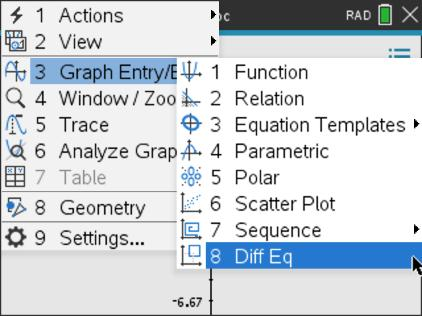
\includegraphics[width=\linewidth]{Pics/1.5.1.jpg} & 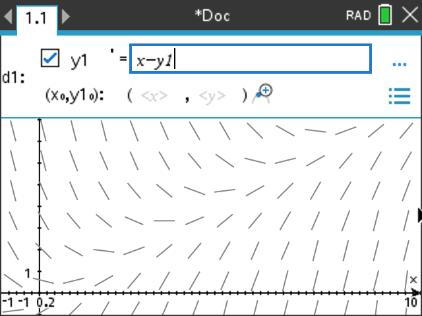
\includegraphics[width=\linewidth]{Pics/1.5.2.jpg} \\
    Select: Menu, 3: Graph Entry/Edit, 8: Diff Eq. & Write down the ODE
  \end{tabular}
\end{table}

\section{Solvability}
\noindent\rule[\linienAbstand]{\linewidth}{\linienDickeDick}
Two solution curves of an ODE cannot cross.


\part{Ordinary Differential Equations}
\section{Analytical methods for first-order ODE’s}
\noindent\rule[\linienAbstand]{\linewidth}{\linienDickeDick}

\subsection{Overview}
\noindent\rule[\linienAbstand]{\linewidth}{\linienDicke}
For some types of explicit first-oder ODE’s there exist analytical solution methods:\\

\textbf{Separable ODE's}\\
We discuss this type of ODE’s in detail. The main reason why separable ODE’s are interesting is the fact that the special cases “Indefinite integral” and “Autonomous ODE” are of this type, and many important examples from applications are autonomous ODE’s.\\

\textbf{Linear ODE's}\\
We discuss linear ODE’s in the following section in the context of the discussion of linear ODE’s of arbitrary order. For linear ODE’s the distinction between homogeneous and inhomogeneous equations is crucial. A homogeneous first-order ODE is separable and can therefore be solved by the standard procedure for separable ODE’s. For inhomogeneous ODE’s, one often arrives at a solution by assuming an ansatz of the form of the inhomogeneity.\\


\subsection{Separable ODE’s}
\noindent\rule[\linienAbstand]{\linewidth}{\linienDicke}
How to find the general solution of a separable ODE is best expalined with an example:\\
We compute the general solution of the ODE
\begin{equation}
  y' = -\frac{x}{y}
\end{equation}
We write the eqution as
\begin{equation}
  \frac{\textup{d}y}{\textup{d}x} = -\frac{x}{y}
\end{equation}
We bring all $x$-dependent terms to the left hand side and all $y$-dependent terms on
the right hand side:
\begin{equation}
  y\:\textup{d}y = -x \:\textup{d}x
\end{equation}
We integrate on both sides and get
\begin{equation}
  \int y\:\textup{d}y = - \int x\:\textup{d}x \Rightarrow \frac{1}{2}y^2 = - \frac{1}{2} x^2 + C, \;\;\; C \in \mathbb{R}
\end{equation}
We solve for y and get
\begin{equation}
  y = \pm \sqrt{K - x^2}, \;\; K \in \mathbb{R}\;\; (\text{where } K = 2C)
\end{equation}

% \textbf{Example of substitution}\\
% We consider the ODE
% \begin{equation}
%   y' = (x + y)^2
% \end{equation}
%
%
% \subsection{Exact ODE’s}
% \noindent\rule[\linienAbstand]{\linewidth}{\linienDicke}

\section{Analytical methods for linear ODE’s}
\noindent\rule[\linienAbstand]{\linewidth}{\linienDickeDick}

\subsection{Overview}
\noindent\rule[\linienAbstand]{\linewidth}{\linienDicke}
We differentiate bewteen first-order linear ODE's and higher-oder ODE's as well as between homogeneous and inhomogeneous ODE's.\\

The general solution of the inhomogeneous ODE is the sum
\begin{equation}
  y = y_h + y_s,
  \label{eq:2.50}
\end{equation}
where $y_h$ is the general solution of the homogeneous ODE and $y_s$ any special solution of the inhomogeneous ODE.

\subsection{First-order linear ODE's}
\noindent\rule[\linienAbstand]{\linewidth}{\linienDicke}
To solve a first-order linear ODE we thus have to find $y_h$ and $y_s$\\
$\mathbf{y_h}$: a homogeneous first-order ODE is separable and can therefore be solved by the standard procedure for separable ODE’s described above.\\
$\mathbf{y_s}$: To find a special solution of and ODE, there are several possibilities. In the case of an ODE with constant coefficients, it usually suffices to choose for $y_s$ an \emph{ansatz of the form of the source term $g(x)$}. In the case of non-constant coefficients, the method \emph{variation of constants} usually works better.\\

\textbf{Example using the ansatz}\\
We solve the ODE
\begin{equation}
  y' + ay = b
\end{equation}
- To determine $y_h$, we integrate the homogeneous ODE
\begin{equation}
  y' + ay = 0
\end{equation}
by separation of variables we obtain the solution
\begin{equation}
  y_h = C \cdot e^{-ax}, \;\; C \in \mathbb{R}.
\end{equation}
- For finding $y_s$ we choose the ansatz in the form of the source term. In this case the source term is constant, $g(x) = b$. Therefore we assume that the special solution $y_s$ is constant as well, i.e. we make an ansatz $y_s = c$. We plug this ansatz into the inhomogeneous ODE and obtain the special solution $y_s$.
\begin{equation}
  y_s'+ay_s = b \;\;\; \Rightarrow \;\;\; y_s = \frac{a}{b}
\end{equation}
The general solution therefore is
\begin{equation}
  y = C \cdot e^{-ax} + \frac{a}{b}, \;\; C \in \mathbb{R}
\end{equation}

\textbf{Ansatz functions for the solution of the inhomogeneous first-order ODE}
\begin{table}[H]
  \begin{tabular}{ll}
    Source term $g(x)$ & Ansatz $y_s$\\
    $g(x) = b_0$ & $y_s = c_0$\\
    $g(x) = b_1x + b_0$ & $y_s = c_1x + c_0$\\
    $g(x) = b_2x^2 + b_1x + b_0$ & $y_s = c_2 x^2 + c_1x + c_0$\\
    $g(x) = \sum_{i = 0}^n b_i x^i$ & $y_s = \sum_{i = 0}^n c_i x^i$\\
    $g(x) = A\;sin(\omega x) + B\;cos(\omega x)$ & $
    \begin{aligned}
      y_s &= C_1sin(\omega x) + C_2 cos(\omega x)\\
      y_s &= Csin(\omega x + \varphi)
    \end{aligned}$\\
    $g(x) = Ae^{bx}$ & $y_s =
    \left\{\begin{matrix}
      \frac{A}{b + a}e^{bx} \;\; \text{ for } b \neq -a\\
      Axe^{-ax} \;\text{ for } b = -a
    \end{matrix}\right.$
  \end{tabular}
\end{table}
In addition, the following rules must be followed:\\
\textbf{Linearity} If $g(x)$ is a linear combination of several source terms, one has to assume as ansatz for $y_s(x)$ a correponding linear combination of several ansatz terms.\\
\textbf{Resonance} If the source term $g(x)$ is itself already a solution of the homogeneous ODE, the correponding ansatz for $y_s$ has to be multiplied with x. So if for example $y_h = Ce^x$, and $g(x) = e^x$, the ansatz $y_s = \mathbf{x} \cdot e^x$ is choosen.\\

\textbf{Example using Variation of constants}\\
The idea behind the variation of constants is to start from the solution $y = K \cdot e^{-F(x)}$ of the homogeneous ODE and plug the ansatz
\begin{equation}
  y = K(x) \cdot e^{-F(x)}
\end{equation}
into the inhomogeneous ODE.\\
As an example we want to solve the inhomogeneous linear ODE
\begin{equation}
  3y' + 5y = \color{violet} 7e^{\frac{1}{3}x} \color{black}.
\end{equation}
- We first find the homogeneous solution $y_h$ by separation of variables.
\begin{equation}
  \frac{1}{y}\textup{d}y = -\frac{5}{3}x \; \textup{d}x
  \;\;\; \Rightarrow \;\;\;
  y_h = \color{blue} e^{\frac{5}{3}x} \cdot K \color{black}
\end{equation}

- Next we calculate the ansatz and its derivative
\begin{equation}
  \begin{split}
      y_s =& \color{blue} e^{-\frac{5}{3}x} \cdot K(x) \color{black}\\
      y_s' =& \color{red} K(x)' e^{-\frac{5}{3}x} + K(x) \cdot -\frac{5}{3} e^{-\frac{5}{3}x} \color{black}
  \end{split}
\end{equation}

- The ansatz is then pluged into the inhomogeneous ODE
\begin{equation}
  3\left(\color{red} K(x)' e^{-\frac{5}{3}x} + K(x) \cdot -\frac{5}{3} e^{-\frac{5}{3}x} \color{black}\right) +
  5\left(\color{blue} e^{-\frac{5}{3}x}\cdot K(x) \color{black}\right) =
  \color{violet} 7e^{\frac{1}{3}x} \color{black}
\end{equation}
- We solve for $K(x)'$ ($K(x)$ usually dissapears)
\begin{equation}
  3 \cdot \color{red} K(x)' e^{-\frac{5}{3}x} \color{black} = \color{violet} 7e^{\frac{1}{3}x} \color{black}
  \;\;\;\Rightarrow \;\;\;
  K(x)' = \frac{7}{3}e^{\frac{1}{3}x + \frac{5}{3}x} = \frac{7}{3}e^{2x}
\end{equation}
- We integrate and find $K(x)$
\begin{equation}
  K(x) = \frac{7}{6}e^{2x}
\end{equation}
- Plugin $K(x)$ into the ansatz we get the special solution $y_s$
\begin{equation}
  y_s = e^{-\frac{5}{3}x} \cdot \frac{7}{6}e^{2x} = \frac{7}{6}e^{\frac{1}{3}x}
\end{equation}
- The solution $y_h + y_s$ is then
\begin{equation}
  y = K \cdot e^{-\frac{5}{3}x} + \frac{7}{6}e^{\frac{1}{3}x}
\end{equation}
If the problem is an initial value problem; plug in values for x and y and solve for $K$.

\subsection{Higher-order linear ODE's}
\noindent\rule[\linienAbstand]{\linewidth}{\linienDicke}
The fact that the solution of an inhomogeneous ODE is the sum of the solution of the homogeneous ODE and the special solution (equation \ref{eq:2.50}) still holds true for higher-order linear ODE's

\textbf{The homogeneous case}\\
The function $y = e^{\lambda x}$ is a solution of the homogeneous ODE if and only if $\lambda$ is a root of the characteristic polynomial, i.e. if
\begin{equation}
  P(\lambda) = 0
\end{equation}
We now have to distinguish between real and complex and between single and multiple roots of the characteristic polynomial.

\textbf{Real Roots}
If $\lambda$ is a real root of $P(\lambda)$ of multiplicity $m$, then the functions
\begin{equation}
  y_1 =e^{\lambda x}, \;   y_2 =xe^{\lambda x} ,...,\;   y_m =x^{m-1}e^{\lambda x}
\end{equation}
are distinct linearly independent solutions. i.e. if $m = 1$ and $\lambda$ is a simple root then $y = C_1\; e^{\lambda x}$ is the solution.\\
Example: The homogeneous ODE
\begin{equation}
  y^{(3)}- 3y'' - 4y' = 0
\end{equation}
has the characteristic polynomial
\begin{equation}
  P(\lambda) = \lambda^3 - 3\lambda^2 - 4\lambda.
\end{equation}
The roots of this polynomial are $\lambda_1 = 0, \lambda_2 = 4, \lambda_3 = -1$, hence the general solution of
the ODE is
\begin{equation}
  y = C_1 + C_2 e^{4x} + C_3e^{-x}
\end{equation}

\textbf{Complex Roots}
If $\lambda = \alpha \pm j\beta$ are two complex roots of $P(\lambda)$ of multiplicity $m$ then
\begin{table}[H]
  \begin{tabular}{ll}
    $y_1 = e^{\alpha x} cos(\beta x)$ &   $y_2 = e^{\alpha x} sin(\beta x)$\\
    $y_3 = xe^{\alpha x} cos(\beta x)$ &   $y_4 = xe^{\alpha x} sin(\beta x)$\\
    \vdots  & \vdots \\
    $y_{2m-a} = x^{m-1}e^{\alpha x} cos(\beta x)$ &   $y_{2m} = x^{m-1}e^{\alpha x} sin(\beta x)$
  \end{tabular}
\end{table}
are m linearly independent solutions.\\
If $m = 1$ and $\lambda_{1,2} = \alpha \pm \beta$ then $y_1 = C_1 e^{ax}cos(\beta x)$ and $y_2 = C_2 e^{ax}sin(\beta x)$ are two linearly
independent solutions.\\
Example: The homogeneous ODE
\begin{equation}
  y'' + y = 0
\end{equation}
has the characteristic polynomial
\begin{equation}
  P(\lambda) = \lambda^2 + 1.
\end{equation}
The roots of this polynomial are $\lambda_1 = j, \lambda_2 = -j$, hence the general solution of the ODE is
\begin{equation}
  y = C_1 cos(x) + C_2 sin(x)
\end{equation}

\textbf{The inhomogeneous case}\\
We now determine special solutions of the inhomogeneous ODE's. The best method for solving such ODE's is as above using an ansatz of the form of the source term, with undetermined coefficients. These coefficients are then determined by plugging the ansatz into the equation.\\
Example: Consider the inhomogeneous ODE
\begin{equation}
  y^{(3)} + y'' + y' + y = 2x + 5
\end{equation}
The general solution of the homogeneous ODE is (The complex roots are $-1, -j, j)$
\begin{equation}
  y_h = C_1 e^{-x} + C_2cos(x) + C_3 sin(x)
\end{equation}
To find a special solution of the inhomogeneous ODE, we choose the ansatz
\begin{equation}
  y_s = b_1x + b_0
\end{equation}
Plugin this into the initial ODE leads to
\begin{equation}
  b_1 + (b_1x + b_0) = 2x + 5
\end{equation}
which leas to the following linear system of equations for a and b
\begin{equation}
  \begin{vmatrix}
        &   & b_1 & = & 2\\
    b_1 & + & b_0 & = & 5
  \end{vmatrix}
  \;\;\; \Rightarrow \;\;\;
  b_1 = 2, \;\;\; b_0 = 3
\end{equation}
The desired special solution hence is
\begin{equation}
  y_s = 2x + 3
\end{equation}
and the general solution therefore is
\begin{equation}
  y = C_1 e^{-x} + C_2cos(x) + C_3 sin(x) + 2x + 3
\end{equation}

\section{Numerical Methods}
\noindent\rule[\linienAbstand]{\linewidth}{\linienDickeDick}
\begin{equation}
  \begin{split}
    h =& t_{k+1} - t_k\\
    t_k =& t_0 + k \cdot h, \;\; k \in \mathbb{N}
  \end{split}
\end{equation}

\subsection{Explicit Eulers Method}
\noindent\rule[\linienAbstand]{\linewidth}{\linienDicke}
\begin{equation}
  \begin{split}
    \dot{x} &= f(t, x)\\
    x_{k+1} &= x_k + h \cdot f(t_k, x_k)
  \end{split}
\end{equation}

\subsection{Implizit Eulers Method}
\noindent\rule[\linienAbstand]{\linewidth}{\linienDicke}
\begin{equation}
  \begin{split}
    x_{k+1} = x_k + h \cdot f(t_{k+1}, x_{k+1})
  \end{split}
\end{equation}

\subsection{Midpoint Method}
\noindent\rule[\linienAbstand]{\linewidth}{\linienDicke}
\begin{equation}
  \begin{split}
    x_{k+\frac{1}{2}} &= x_k + \frac{h}{2} \cdot f(t_k, x_k)\\
    x_{k+1}           &= x_k + h \cdot f(t_{k} + \frac{h}{2}, x_{k+\frac{1}{2}})
  \end{split}
\end{equation}

\subsection{Heun Method}
\noindent\rule[\linienAbstand]{\linewidth}{\linienDicke}
\begin{equation}
  \begin{split}
    k_1 &= f(t_k, x_k)\\
    k_2 &= x_k + h \cdot f(t_k, x_k)\\
    x_{k+1} &= x_k + \frac{h}{2}(k_1 + k_2)
  \end{split}
\end{equation}

\subsection{Runge-Kutta Method of Fourth Order}
\noindent\rule[\linienAbstand]{\linewidth}{\linienDicke}
\begin{equation}
  \begin{split}
    k_1 &= f(t_k, x_k)\\
    k_2 &= f(t_k + \frac{h}{2}, x_k + \frac{h}{2}k_1)\\
    k_3 &= f(t_k + \frac{h}{2}, x_k + \frac{h}{2}k_2)\\
    k_4 &= f(t_k + h, x_k +h \; k_3)\\
    x_{x+1} &= x_k + \frac{h}{6}(k_1 + 2k_2 + 2k_3 + k_4)
  \end{split}
\end{equation}

\begin{figure}[H]
  \centering
  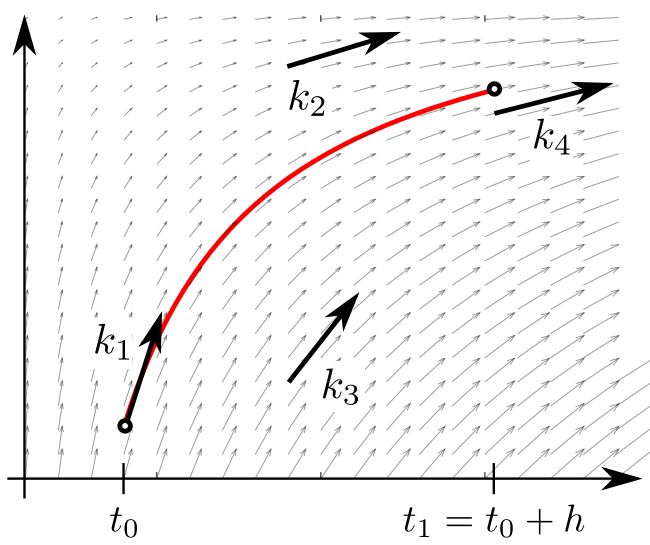
\includegraphics[width=0.5\linewidth]{Pics/runge.png}
\end{figure}

\subsection{Error Order}
\noindent\rule[\linienAbstand]{\linewidth}{\linienDicke}
The (global) error orders of the various methods discussed before are:
\begin{itemize}
  \item Explicit Euler method: $p = 1$
  \item Midpoint rule: $p = 2$
  \item Heun method: $p = 2$
  \item Classical Runge-Kutta method: $p = 4$
\end{itemize}
The higher the error order of a method, the smaller thus the error is which one has to take into account by using the method. On the other hand, the computational cost for the preciser methods is often higher as well.


\part{System of Differential Equations}
\section{Analytical methods for linear systems}
\noindent\rule[\linienAbstand]{\linewidth}{\linienDickeDick}
By the definition given above, by a system of ODE’s we mean the following system of explicit firstoder ODE’s:
\begin{equation}
  \begin{matrix}
    \dot{x}_1 & = & f_1(t, x_1, ..., x_n)\\
    \vdots  &  & \vdots \\
    \dot{x}_n & = & f_n(t, x_1, ..., x_n)
  \end{matrix}
\end{equation}

\subsection{Overview}
\noindent\rule[\linienAbstand]{\linewidth}{\linienDicke}
A system of linear first-order ODE’s has the form
\begin{equation}
  \begin{matrix}
    \dot{x}_1 & = & a_{11}(t)x_1 + ... + a_{1n}(t)x_n + b_1 (t)\\
    \vdots  &  & \vdots \\
    \dot{x}_n & = & a_{n1}(t)x_1 + ... + a_{nn}(t)x_n + b_n (t)
  \end{matrix}
\end{equation}
or in matrix-vector notation
\begin{equation}
  \dot{\mathbf{x}} = A(t)\mathbf{x}+\mathbf{b}t
\end{equation}
The general solution of the inhomogeneous system is the sum
\begin{equation}
  \mathbf{x} = \mathbf{x}_h+ \mathbf{x}_s
\end{equation}
where $x_h$ is the general solution of the homogeneous system and $x_s$ any special solution of the inhomogeneous system.\\

The set of solutions of the homogeneous system is an n-dimensional vector space. This is equivalent to the following two statements:\\
 - Any linear combination of solutions is again a solution, i.e. if $x_1$ and $x_2$ are solutions, then $C_1x_1 + C_2x_2$ is also a solution for any $C_1, C_2 \in \mathbb{R}$\\
 - There exist precisely $n$ linearly independent solution $x_1, . . . , x_n$. Such a set $\{x_1, . . . , x_n\}$ of linearly independent solutions is also called a \emph{fundamental system of solutions}. Algebraically, a fundamental system thus is a basis of the vector space of solutions.\\

\subsection{Homogeneous linear systems}
\noindent\rule[\linienAbstand]{\linewidth}{\linienDicke}
Since in the scalar case the solution of a homogeneous linear ODE is given by $x = e^{at}$, we try in the vectorial case an ansatz of the form
\begin{equation}
  \mathbf{x} = e^{\lambda t} \cdot c =
  \begin{pmatrix}
    e^{\lambda t}c_1\\
    \vdots\\
    e^{\lambda t}c_n
  \end{pmatrix}
\end{equation}
Plugging the ansatz into the ODE leads to $e^{\lambda t}\lambda c = e^{\lambda t} Ac$ and we thus get for $\lambda$ and $c$ the equation
\begin{equation}
  A\mathbf{c} = \lambda \mathbf{c}
\end{equation}
This precisely means that $c$ is an \emph{eigenvector} of $A$ to the \emph{eigenvalue} $\lambda$.\\

\textbf{Example}\\
We compute the general solution of the homogeneous system
\begin{equation}
  \begin{split}
    \dot{x}_1 &= 2x_1 - x_2\\
    \dot{x}_2 &= -x_1 + 2x_2
  \end{split}
\end{equation}

or in the form $\dot{\mathbf{x}} = A\mathbf{x}$ with
\begin{equation}
  \mathbf{x}(t) = \begin{pmatrix}
    x_1(t)\\
    x_2(t)
  \end{pmatrix}
  , \;\; A = \begin{pmatrix}
      2 & -1\\
      -1 & 2
  \end{pmatrix}
\end{equation}

The matrix $A$ has the eigenvaluess $\lambda_1 = 1, \lambda_2 = 3$ with corresponding eigenvectors $v_1 = \binom{1}{1}, v_2 = \binom{1}{-1}$. Hence the general solution $\mathbf{x}(t)$ of the homogeneous system is
\begin{equation}
  \mathbf{x}(t) = \begin{pmatrix}
    x_1(t)\\
    x_2(t)
  \end{pmatrix} = C_1 \begin{pmatrix} 1 \\ 1 \end{pmatrix} e^t+
  C_2 \begin{pmatrix} 1 \\ -1 \end{pmatrix} 3^{3t}
\end{equation}

\subsection{Inhomogeneous linear systems}
\noindent\rule[\linienAbstand]{\linewidth}{\linienDicke}


\part{Dynamical Systems}

\end{multicols}
\end{document}
